\chapter{Fundamentos e Revisão de Literatura}
\label{chap:fundamentacao}
A definição de alguns termos, técnicas e/ou ferramentas se faz necessária para o entendimento deste estudo. A conceituação de sensibilidade ao contexto é importante, uma vez que se constitui da técnica de obtenção dos dados. 
%Como complemento à sensibilidade ao contexto apresenta-se o ZooKeeper, ferramenta utilizada para transmissão dos dados coletados. 
Além disso, é relevante que exista a compreensão de como funcionam o Apache Hadoop, seu escalonamento e o paradigma de programação utilizado, bem como dos trabalhos já realizados em áreas correlatas a este trabalho.

%-------------------------------------------------------------------

\section{MapReduce}
O paradigma de programação MapReduce é, geralmente, associado com implementações que processam e geram grandes conjuntos de dados. Neste paradigma, todo processamento é dividido em duas etapas, a etapa de Map e a de Reduce, que são inspiradas pelas funções de mesmo nome em linguagens funcionais. Como consequência da divisão em duas etapas, o resultado da primeira é a entrada da segunda e esta transferência de dados é baseada em pares de chave e valor, o que torna possível expressar uma vasta gama de tarefas reais por meio deste paradigma~\cite{Dean}.

O \textit{workflow} padrão de uma aplicação MapReduce inicia com a entrada de dados, que será dividida em \textit{n} partes, sendo que cada parte será processada individualmente por uma tarefa Map. O resultado das tarefas Map será transmitido na forma de pares chave e valor, que serão utilizados como entrada para as tarefas de Reduce. Por fim, as tarefas de Reduce irão receber todos os pares com determinada chave e aplicar um algoritmo sobre os pares, fornecendo uma saída inteligível~\cite{BookHadoop}.

\section{Apache Hadoop}
O \textit{framework} Apache Hadoop origina-se de outro projeto da Apache, o Apache Nutch \cite{Nutch}, que iniciou em 2002 como um motor de buscas de código livre porém, logo encontrou problemas devido a sua arquitetura. Quando a Google publicou um artigo em 2003 descrevendo a arquitetura utilizada no seu sistema de arquivos distribuídos, chamado GFS (\textit{Google File System}), os desenvolvedores do Nutch notaram que uma arquitetura semelhante resolveria seus problemas de escalabilidade. A implementação da ideia foi iniciada em 2004 e o resultado foi nomeado \textit{Nutch Distributed Filesystem} (NDFS). Contudo, à medida em que o projeto se desenvolvia, o propósito original do Nutch era deixado em segundo plano, o que culminou na criação de um novo projeto em 2006, denominado Apache Hadoop, com o propósito de facilitar o processamento distribuído através do paradigma MapReduce.

\subsection{Arquitetura geral do Apache Hadoop}
O \textit{framework} Apache Hadoop é organizado em uma arquitetura de mestre-escravo que possui dois serviços principais: o serviço de armazenamento (HDFS - Hadoop Distributed File System) e o de processamento (YARN - Yet Another Resource Negotiator), os quais podem ser vistos na Figura \ref{fig:ArquiteturaHadoop}.

\begin{figure}[!ht]
\centering
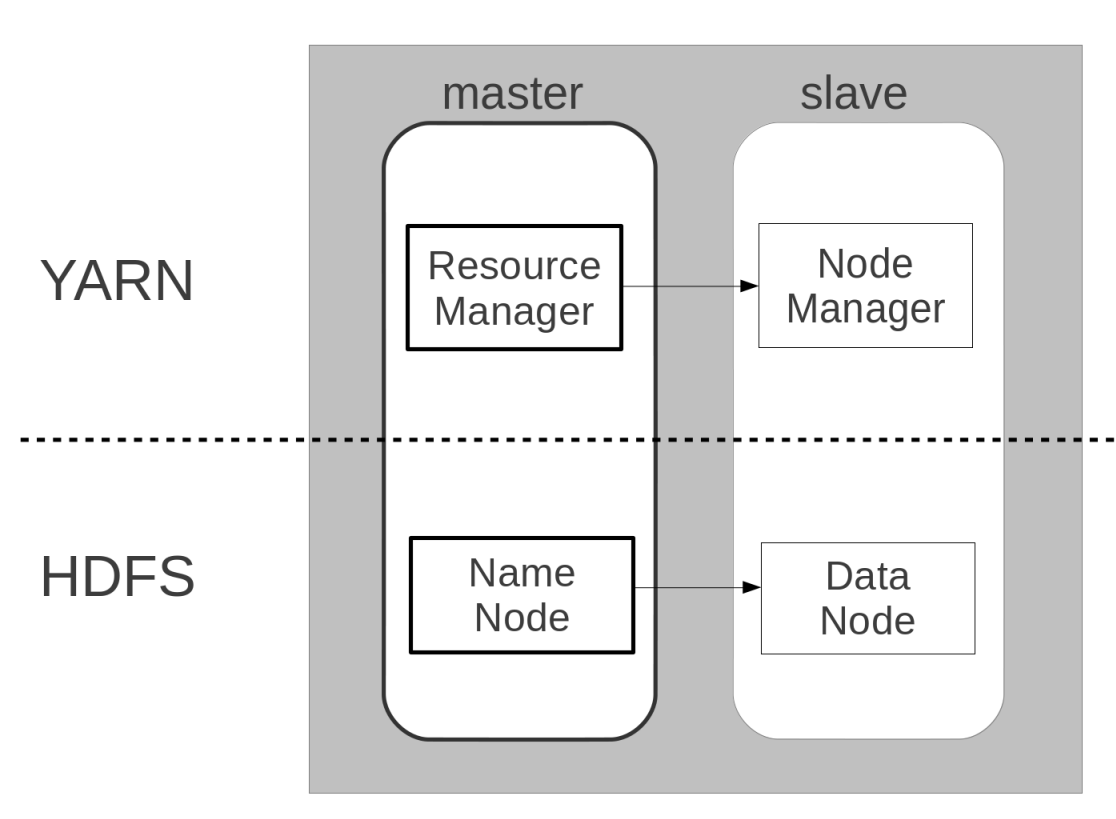
\includegraphics[width=0.7\textwidth]{figuras/Figura08-HadoooArchGeral.png}
\caption{Arquitetura geral do Apache Hadoop}
\label{fig:ArquiteturaHadoop}
\end{figure}

Nesta figura, é possível notar a existência de 4 componentes do \textit{framework}. Os componentes acima da linha pontilhada pertencem ao YARN, sendo o Resource Manager e o Node Manager os serviços mestre e escravo respectivamente. O HDFS é composto pelos componentes abaixo da linha pontilhada, sendo o Name Node e o Data Node os serviços mestre e escravo respectivamente.

\subsubsection{HDFS}
Grande parte do ganho de desempenho oferecido pelo Hadoop decorre do comportamento de levar o processamento até os dados, ou seja, todo processamento é feito com dados locais. Para realizar esta tarefa, o Name Node mantém informações de quais partes de quais arquivos estão em cada Data Node, ou seja, todos os arquivos estão divididos em um grande HD distribuído e o mestre sabe exatamente quais blocos cada escravo possui. Dessa forma, cada nó executa tantos Maps ou Reduces quanto a quantidade de arquivos locais permitir, diminuindo a necessidade de utilizar a rede para transferência de arquivos e deixando-a disponível para ser utilizada para a transferência dos resultados que são os dados já reduzidos. Um problema dessa abordagem é que o Hadoop possui uma latência muito alta, sendo desaconselhável o uso do Hadoop em aplicações críticas ou de tempo real \cite{BookHadoop}. A Figura \ref{fig:ArqHDFS} apresenta um esquema básico da arquitetura do HDFS.

\begin{figure}[!hbt]
   \centering
   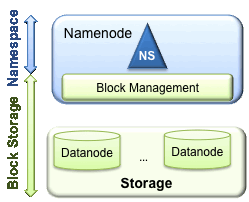
\includegraphics[width=8cm]{figuras/Figura07-HDFS.png}
   \caption{Arquitetura geral do HDFS \cite{HDFS}}
   \label{fig:ArqHDFS}
\end{figure}

\subsubsection{YARN}
Sendo o componente do Apache Hadoop responsável pela execução do \emph{MapReduce}, o YARN realiza tarefas de gerenciamento e execução do processamento. Um dos objetivos do YARN é tornar a tarefa de processamento totalmente independente das tarefas de armazenamento, possibilitando que o \textit{cluster} seja utilizado em conjunto com outras ferramentas que não utilizem o paradigma MapReduce \cite{Vavilapalli}. A Figura \ref{fig:ArqYARN} apresenta um esquema básico da arquitetura do YARN, onde é possível observar dois novos componentes do YARN.

\begin{figure}[!hbt]
   \centering
   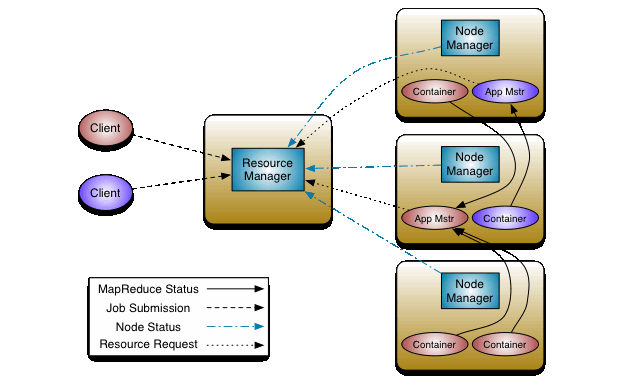
\includegraphics[width=12cm]{figuras/Figura06-YarnArch.png}
   \caption{Arquitetura geral do YARN \cite{YARN}}
   \label{fig:ArqYARN}
\end{figure}

O primeiro é o Application Master (apresentado na imagem como App Mstr), um componente do Node Manager que possui o papel de um escalonador interno de cada aplicação , sendo também referenciado como escalonador de tarefas. Considera-se que tarefas sejam uma fração do processamento das aplicações, ou seja, cada tarefa de Map ou Reduce corresponde a uma das divisões que serão processadas em paralelo. É importante não confundir este componente com o escalonador de aplicações, o qual pertence ao Resource Manager e pode ser melhor compreendido com a leitura da Seção \ref{sec:HadSched}. O outro componente presente na figura é o Container, o qual representa a alocação de recursos em um nó qualquer do \textit{cluster}. A importância do Container vem do fato de que todas as tarefas são executadas em uma de suas instâncias.

É importante notar que existem 2 instâncias de Application Master na figura e que elas estão, assim como os clientes e os containers, coloridas de rosa ou roxo para indicar que pertencem à mesma aplicação, ou seja, o cliente rosa lançou uma aplicação que possui o Application Master e mais 3 \textit{containers} de processamento. Nota-se também que o Resource Manager recebe informações tanto dos clientes quanto dos Node Managers e Application Masters, centralizando todas elas para um controle dos recursos disponíveis.

\subsubsection{Configuração do ambiente de execução do Hadoop}
Uma característica importante do Hadoop tem relação com sua configuração. O Hadoop utiliza uma série de arquivos em cada um dos nós do \textit{cluster} para definir sua configuração. Estes arquivos, em formato XML, contêm nomes de parâmetros e seus valores que influenciam o comportamento do \textit{framework} no \textit{cluster}. Os arquivos são denominados: \textit{core-site.xml, yarn-site.xml, mapred-site.xml} e \textit{hdfs-site.xml}. Cada um destes arquivos possui propriedades de um serviço do Hadoop, como exemplo o arquivo \textit{hdfs-site.xml} é responsável pela configuração do HDFS na máquina e permite a configuração de parâmetros como o tamanho dos blocos e a replicação dos dados.

É importante salientar que, para a execução distribuída, ao menos algumas propriedades mais simples dos arquivos de cada nó, seja este mestre ou escravo, devem ser configuradas. No caso do administrador desejar fazer uma configuração mais específica de cada nó escravo, ele deverá editar as propriedades nos arquivos de cada um dos nós. Caso o administrador não queira configurar os nós escravos, eles irão executar com base nos valores \textit{default}, contudo esta decisão irá, provavelmente, afetar o desempenho do \textit{cluster} devido à má configuração.

A utilização de valores \textit{default} facilita a implementação, porém cria alguns problemas na utilização do \textit{framework} em situações diferentes da suposição inicial de um \textit{cluster} dedicado e homogêneo. Em um \textit{cluster} homogêneo, a configuração é simples, uma vez que todos os nós possuem a mesma configuração de recursos. Contudo, em alguns casos, é possível que o \textit{cluster} não seja homogêneo e que a configuração torne-se mais complexa dependendo da quantidade de configurações diferentes existentes no \textit{cluster}.

A configuração estática pode tornar-se ainda mais problemática quando o \textit{cluster} é compartilhado. Neste caso, a informação que estava correta no arquivo XML pode, em algum momento, ficar inconsistente com a realidade devido à utilização do \textit{cluster} para a execução de algo além de aplicações MapReduce.
 



%-------------------------------------------------------------------

\section{Escalonadores para o Hadoop}
\label{sec:HadSched}
Apesar de existirem dois níveis de escalonamento no Hadoop, escalonamento de aplicações e de tarefas, este trabalho de mestrado aborda apenas o escalonamento de aplicações. O escalonador de aplicações gerencia qual será a primeira aplicação a receber um \textit{container} para seu escalonador de tarefas e quais serão os escalonadores de tarefa que receberão recursos para execução \cite{BookHadoop}. O Hadoop já inclui alguns escalonadores que oferecem maneiras diferentes para a realização do escalonamento de aplicações. Para alterar o escalonador utilizado é necessário alterar uma propriedade no arquivo \textit{yarn-site.XML} e reiniciar o Resource Manager.

Dentre os escalonadores incluídos no Hadoop, o mais simples é o Hadoop Internal Scheduler que utiliza o algoritmo FIFO e tem bom desempenho em \textit{clusters} onde não existe competição por recursos. Este escalonador suporta até 5 níveis de prioridade, porém a decisão da próxima aplicação a ser executada sempre levará em consideração a hora de submissão.

Um pouco mais complexo que o Internal Scheduler, o Fair Scheduler é utilizado, principalmente, para o processamento de lotes de aplicações pequenas e rápidas, opera baseado em um escalonamento de dois níveis e possui o objetivo de realizar uma divisão justa dos recursos. O primeiro nível realiza o escalonamento na forma de filas para cada usuário ativo, dividindo os recursos do \textit{cluster} igualitariamente entre as filas. Enquanto isso, o segundo nível realiza o escalonamento dentro de cada fila da mesma forma que o Internal Scheduler \cite{FairScheduler}. 

A terceira opção, e também o padrão do Hadoop nas últimas versões, é o Capacity Scheduler, o qual foi projetado para a utilização compartilhada do Hadoop e busca a maximização do \textit{throughput} e da utilização do \textit{cluster}. Seu funcionamento baseia-se em garantias mínimas de capacidade para os usuários, ou seja, qualquer usuário terá sempre uma garantia mínima de recursos para utilização. Porém, quando algum usuário está com seus recursos ociosos, o escalonador repassa a capacidade deste usuário  para aqueles que estão utilizando o \textit{cluster}. Esta estratégia fornece elasticidade com um bom custo benefício, uma vez que diferentes organizações possuem diferentes horários de pico para o processamento de informações. Este escalonador é capaz de rastrear os recursos registrados no Resource Manager, embora esta informação possa não ser consistente com a realidade, e monitorar quais deles estão livres e quais estão sendo utilizados pelo \textit{framework} \cite{CapacityScheduler}.

%TODO explicar o escalonamento do CapacityScheduler

A existência destes escalonadores adiciona flexibilidade no gerenciamento do \textit{framework}. Apesar disso, os escalonadores disponíveis não detectam nem reagem à dinamicidade e heterogeneidade do ambiente. Para a utilização do Hadoop em ambientes pervasivos é necessário que exista uma capacidade de adaptação neste componente.




%-------------------------------------------------------------------

\section{Trabalhos Relacionados}
%TODO adicionar os novos trabalhos que não existiam no TG
Existem outras implementações de escalonadores além dos três escalonadores já inclusos no Hadoop, nas quais é possível identificar diversas propostas de adaptação. Cada proposta possui métodos e objetivos específicos, tornando um estudo sobre estas implementações interessante como ponto de partida para a proposta deste trabalho de mestrado. Logo, buscou-se identificar quais técnicas foram mais utilizadas e quais os tipos de adaptação mais explorados nestes escalonadores. 

%A seguir encontram-se os trabalhos relacionados e um breve resumo sobre a proposta, método e objetivos esperados com a adaptação.


Os autores do escalonador CASH (\emph{Context Aware Scheduler for Hadoop} - Escalonador Sensível ao Contexto para o Hadoop) \citet{CASH} têm o objetivo de melhorar o rendimento geral do \emph{cluster}. O trabalho utiliza a hipótese de que grande parte das aplicações são periódicas e executadas no mesmo horário, além de possuírem características de uso de CPU, rede, disco, etc., semelhantes. O trabalho ainda levou em consideração que, com o passar do tempo os nós tendem a ficar mais heterogêneos. Baseados nestas hipóteses e com objetivo de melhorar o desempenho geral, foi implementado um escalonador que classifica tanto as aplicações como as máquinas com relação ao seu potencial de CPU e E/S, podendo então distribuir as aplicações para máquinas que possuem uma configuração apropriada para sua natureza.

No trabalho \textit{A Dynamic MapReduce Scheduler for Heterogeneous Workloads} (Um Escalonador de MapReduce Dinâmico para Cargas de Trabalho Heterogêneas) \citet{DMRSHW}, os autores utilizaram a técnica de classificar as aplicações e máquinas de acordo com a quantidade/capacidade de E/S ou CPU. Assim como no CASH, o principal objetivo foi melhorar o desempenho no \textit{cluster}. Uma das diferenças, no entanto, é que esta implementação utiliza um escalonador com três filas.

Semelhante às propostas anteriores, a proposta COSHH (\textit{A Classification and Optimization based Scheduler for Heterogeneous Hadoop Systems} - Um Escalonador Baseado em Classificação e Otimização para Sistemas Heterogêneos do Hadoop) \citet{COSHH} utiliza a classificação das aplicações e máquinas em classes e busca por pares que possuam a mesma classe. Esta busca é feita por um algoritmo que reduz o tamanho do espaço de busca para melhorar o desempenho. O objetivo desta solução é a melhora do tempo médio em que as aplicações são completadas, além de oferecer um bom desempenho quando somente a fatia mínima de recursos for utilizada e, ainda, proporcionar uma distribuição justa.
%O artigo não informa quais informações são utilizadas para a classificação. 

O escalonador LATE (\textit{Longest Approximation Time to End} - Aproximação do Tempo de Término mais Longo) \citet{LATE}, utiliza como informação de contexto o tempo estimado de término da tarefa com base em uma heurística que relaciona tempo decorrido e \textit{score} -- um valor que indica quanto do processamento já foi realizado. Essa informação também é utilizada para gerar um limiar que aponte quando a lentidão de uma tarefa indica sintomas de erros e, a partir desta informação, iniciar uma tarefa especulativa em outra máquina possivelmente mais rápida. Este trabalho teve como objetivo reduzir o tempo de resposta em \textit{clusters} grandes que executam muitas aplicações de pequena duração.

Outro trabalho que utiliza a ideia de mensuração do progresso de uma tarefa é o SAMR (\textit{A Self-adaptative MapReduce} - MapReduce Auto Adaptativo) \citet{SAMR}. Nesta implementação, a informação de contexto é referente ao cálculo do progresso de uma tarefa com objetivo de identificar se o lançamento de uma tarefa especulativa é necessário ou não. Esta solução apresenta como diferencial o cálculo do progresso, o qual varia de acordo com informações do ambiente em que a tarefa está sendo executada. O principal objetivo do trabalho foi reduzir o tempo de execução das tarefas. As informações do ambiente utilizadas para a tomada de decisão consistem de informações históricas contidas em cada nó, e a decisão é tomada após um ajuste do peso de cada estágio do processamento.


A proposta dos autores do \textit{Quincy} \citet{Quincy} difere-se de todos os outros trabalhos, pois possui um escopo muito maior e visa tanto o \textit{Hadoop} como outras ferramentas. O trabalho teve como objetivo a melhora do desempenho geral de um \textit{cluster}, e utilizou a distribuição de recursos como informação de contexto para alcançá-lo. A contribuição do trabalho foi modificar a maneira tradicional de tratamento da distribuição dos recursos. A solução proposta mapeia os recursos em um grafo de capacidades e demandas, para então calcular o escalonamento ótimo a partir de uma função global de custo.

A proposta \textit{Improving MapReduce Performance through Data Placement in heterogeneous Hadoop Clusters} (Melhorando o Desempenho do MapReduce em Clusters Heterogêneos com Hadoop Através da Localização dos Dados) \citet{IMRPDPHHC}, busca melhorar o desempenho de aplicações CPU-bound através da melhor distribuição destes dados. Esta solução utiliza principalmente a localidade dos dados como informação para tomada de decisões. O ganho de desempenho é dado pelo rebalanceamento dos dados nos nós, deixando nós mais rápidos com mais dados. Isso diminui o custo de tarefas especulativas e de transferência de dados pela rede.

Outra proposta que buscou um rebalanceamento de carga foi \citet{Sandholm2009}, porém esta proposta utilizou-se de uma abordagem diferente. Neste trabalho o rebalanceamento de carga foi alcançado através de um sistema baseado na lei de oferta e demanda, o qual permite a cada usuário influenciar diretamente o escalonamento por meio de um parâmetro chamado taxa de gastos. Este parâmetro indica qual a prioridade da aplicação, sendo que, em horários de maior concorrência a taxa de gasto será maior. O principal objetivo desta proposta foi permitir um compartilhamento de recursos dinâmico baseado em preferências configuradas pelos próprios usuários.

Embora não relacionado com escalonamento, o trabalho \citet{Li} propõe uma ferramenta de auto configuração que, em partes, assemelha-se com a proposta do presente estudo. Entretanto, a proposta de Li é baseada em aprendizagem de máquina para a auto configuração de alguns parâmetros chave do Hadoop e apresenta execuções até 10 vezes mais rápidas após a otimização dos parâmetros. Já a proposta deste estudo busca melhorar a informação disponível para que o escalonamento seja adaptável ao compartilhamento do ambiente.

Nota-se que, no geral, as propostas de melhora da adaptabilidade apresentadas pelos trabalhos utilizaram, principalmente, a técnica de rebalanceamento de carga entre nós de diferentes capacidades. Ainda, é possível notar que os trabalhos, em sua maioria, seguem três opções:

\begin{enumerate}
	\item Classificação dos nós e das aplicações de acordo com sua capacidade (CPU ou E/S) seguido de um algoritmo que delega aplicações para nós do mesmo tipo;
	\item Modificação da tomada de decisão sobre o lançamento ou não de uma tarefa especulativa através de novas heurísticas;
	\item Redistribuição dos dados para que mais dados sejam armazenados em nós mais rápidos.
\end{enumerate}

Ainda que a opção 3 assemelhe-se com a opção 1, é importante diferenciar a natureza delas. Enquanto a opção 1 classifica os nós em diversas categorias, a opção 3 apenas delega mais dados e, consequentemente, mais tarefas aos nós mais rápidos. Embora pareça uma solução mais simples, ela evita transferência de dados pela rede, o que aconteceria caso a divisão dos dados para os nós fosse igualitária. No caso dos nós receberem uma quantidade igual de dados inicialmente, os nós mais rápidos terminariam o processamento primeiro e ficariam ociosos até que algum dado fosse transferido para eles.
%
%\newpage
%
%\section{TABELA}
%%Tabela dos casos
%\begin{table}[!h]
%	\centering
%	\begin{tabular}{|p{3.0cm}|p{6.0cm}|p{6.0cm}|}
%		\hline
%		Situação & Default & Trabalho \\
%		\hline
%		Falha nó (morto) & perde tasks (precisa reiniciar quando tiver recursos) e desregistra NM (diminui recursos) & Idem default\\
%		\hline
%		Novo nó (registro) & registar novo NM. Aumenta recursos e escalona tasks que estavam esperando & Idem default\\
%		\hline
%		Nó inicia compartilhamento (- recurso) & \textbf{não reage}, continua alocando containers como se estivesse tudo disponível & \textbf{diminui o recurso do nó. Não afeta containers já alocados, mas só irá alocar quando possuir recurso disponível}\\
%		\hline
%		Nó termina compartilhamento (+ recurso) &\textbf{não reage}, se o nó já estava configurado para utilizar apenas uma parte ele não irá passar a ocupar todos recursos & \textbf{aumenta o recurso do nó. Inicia nova rodada de escalonamento, é como se um novo nó entrasse}\\
%		\hline
%		Cluster heterogêneo & tem que alterar as propriedades dos recursos no XML de todos escravos refletindo as configurações dos nós. Caso contrário existirão nós sobrecarregados ou subutilizados. & Cada nó tera a informação correta. Ganho de desempenho por não sobrecarregar nem subutilizar.\\
%		\hline
%		
%	\end{tabular}
%	\caption{tabela de casos}
%	\label{tab:memory allocation}
%\end{table}
%
%%Tabela dos testes
%\begin{table}[!h]
%	\centering
%	\begin{tabular}{|p{2.5cm}|p{3.5cm}|p{4.5cm}|p{4.0cm}|}
%		\hline
%		Teste & Representa.. & Metodologia & Ponto fraco\\
%		\hline
%		Enganar escalonador para achar que tem mais recursos & cluster compartilhado no momento do início da utilização por outro usuário & inicia x nós com recursos informados dobrados, atualiza durante a primeira leva de containers para valor correto & desta forma é necessário utilizar apenas x/2 nós em relação ao caso A. Pode confundir com um caso de falha de nós\\
%		\hline
%		Nó compartilhado de verdade com informação errada (overload)& cluster compartilhado no momento do início da utilização por outro usuário & reduzir algum recurso de forma que fique indisponível durante a execução. Opções: baloon(MV) - memória, thread - cpu & como garantir que a memória/cpu estará realmente indisponível? quantidade de trabalho extra para realizar o teste\\
%		\hline
%		Enganar escalonador para achar que tem menos recursos & cluster compartilhado no momento do fim da utilização por outro usuário & inicia x nós com recursos informados de x/2, atualiza durante a primeira leva de containers para valor correto & Caso muito improvável, administrador configura o cluster para o Hadoop utilizar apenas uma parte dos recursos dos nós.\\
%		\hline
%		Nó compartilhado de verdade com informação errada (underload)& cluster compartilhado no momento do fim da utilização por outro usuário & reduzir algum recurso de forma que fique indisponível antes do início e torná-lo disponível durante execução. Opções: baloon(MV) - memória, thread - cpu & como garantir que a memória/cpu estará realmente indisponível? quantidade de trabalho extra para realizar o teste\\
%		\hline
%		Teste completo inicia e termina compartilhamento em momentos diferentes durante execução & cluster compartilhado & Inicia com 75\% disponível, reduz recurso durante execução de forma que fique sobrecarregado e aumenta recurso durante execução de forma que fique sub utilizado. Opções: {várias combinações} possíveis de \% & Só é possível fazer sem enganar o cluster. Precisa dos outros testes com controle de recursos funcionando\\
%		\hline
%	\end{tabular}
%	\caption{tabela de testes}
%	\label{tab:memory allocation2}
%\end{table}
